\section{Аналіз та вибір навігаційного забезпечення}

Задача створення комплексної навігаційної системи на базі супутникової та інерціальної 
систем навігації для визначення координат місцеположення рухомого об'єкта, передбачає 
попередній аналіз існуючих варіантів компонентів комплексної навігаційної системи, тобто 
варіантів побудови супутникової й  інерціальної систем навігації та вибір за певними критеріями найбільш оптимальних. 


\subsection{Аналіз і вибір варіанта супутникової навігаційної системи }

На сьогодні має сенс розглядати лише дві супутникові навігаційні системи : GPS (Global Positioning System), 
ГЛОНАСС (Глобальна Навігаційна Супутникова Система).

Двадцять чотири супутники системи GPS знаходяться на 12-годинних орбітах висотою 
metricconverterProductID20 146 км20 146 км із нахиленням орбіти, рівним 55. Таким чином, 
у будь-якій крапці земної кулі в межах прямої видимості мається не менш чотирьох супутників 
у конфігурації, сприятливої для місцевизначення.

Система заснована на обчисленні відстані від користувача до супутника за обмірюваним часом 
від передачі сигналу супутником до прийому цього сигналу користувачем.

Глобальна Навігаційна Супутникова Система (ГЛОНАСС)\textbf{ }- це сума унікальних 
технологій, плід багаторічної праці російських конструкторів і вчених. Вона складається 
з 24 супутників, що, знаходячись у заданих крапках на високих орбітах, безупинно випромінюють 
убік Землі спеціальні навігаційні сигнали. Люба людина або транспортний засіб, оснащені 
спеціальним приладом для прийому й обробки цих сигналів, можуть з високою точністю в 
будь-якій крапці Землі і навколоземного простору визначити власні координати і швидкість 
руху, а також здійснити прив'язку до точного часу.

У складі сучасної супутникової радіонавігаційної системи\textbf{ }(СРНС) типу ГЛОНАСС і 
GPS функціонують три основні підсистеми:

\begin{enumerate}

 


\itemПідсистема космічних апаратів (ПКА), що складається з навігаційних супутників (НС) 
(мережа навігаційних супутників - космічний сегмент). ПКА СРНС складається з визначеного 
числа навігаційних супутників. Основні функції НС --- формування і випромінювання 
радіосигналів, необхідних для навігаційних визначень споживачів СРНС, контролю бортових 
систем супутника підсистемою контролю і керування СРНС. Відповідні характеристики сигналів 
НС і способи їхньої обробки дозволяють проводити навігаційні виміри з високою точністю.

 \item Підсистема контролю і керування (ПКК) (наземний командно-вимірювальний комплекс (КВК)) - 
сегмент керування. ПКК являє собою комплекс наземних засобів (КВК), що забезпечують 
спостереження і контроль за траєкторіями руху НС, якістю функціонування їхньої апаратури, 
керування режимами її роботи і параметрами супутникових радіосигналів, складом, обсягом і 
дискретністю переданої із супутників навігаційної інформації та ін.

 \itemАпаратура споживачів (АС) СРНС (прийомоіндикатори (ПІ)) - сегмент споживачів.
Апаратура споживачів призначена для визначення просторових координат, вектора швидкості, 
часу й інших навігаційних параметрів у результаті прийому й обробки радіосигналів багатьох 
навігаційних супутників (НС).

\end{enumerate}
На вхід ПІ надходять сигнали від НС, що знаходяться в зоні радіо видимості. Оскільки для 
рішення навігаційної задачі необхідно вимірити псевдодальності і псевдошвидкості відносно, 
як мінімум, чотирьох НС, то ПІ повинний бути багатоканальним (більш 24 у сполучених ГЛОНАСС і GPS ).

Сучасні ПІ є аналого-цифровими системами, що здійснюють аналогову і цифрову обробку 
сигналів. Перехід на цифрову обробку здійснюється на одній із проміжних частот, при 
цьому має місце тенденція до підвищення цієї проміжної частоти.

Основа типового варіанту ПІ -- два конструктивно роздільних блоків: антенний блок (АБ) та 
прийомообчислювач (ПО), які призначені для прийому й обробки навігаційних сигналів 
супутників з метою визначення необхідної споживачам інформації (просторово-тимчасових 
координат, напрямки і швидкості і т.п.).

В антенному блоці (рис. \ref{fig:ant_sns}) сукупність сигналів НС, прийнятих антеною, попередньо 
підсилюється і фільтрується по всій смузі несучих частот НС у попередньому підсилювачі 
(ПП) зі смуговим фільтром ( СФ). 

\begin{figure}[here]
\centering
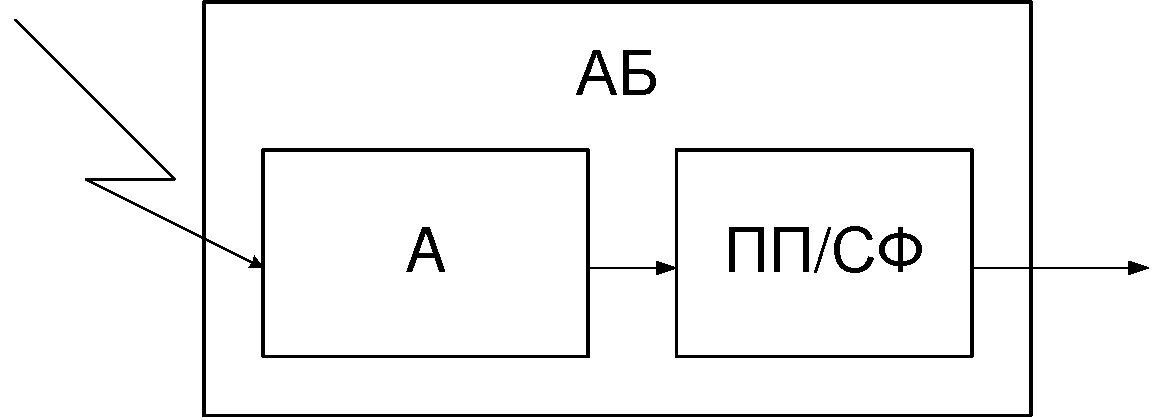
\includegraphics[scale=0.4]{ant_sns}
\caption{Схема антенного блоку СНС}
\label{fig:ant_sns}
\end{figure} 


Прийомообчислювач виконаний у вигляді блоку, у якому розташовані модулі вторинних 
джерел живлення і плати --- прийомокорелятора, навігаційного обчислювача та інтерфейсного 
пристрою (рис. \ref{fig:sns}). Вхід ПО через фідерну лінію з'єднаний з виходом антенного блоку. 
В аналоговому приймачі АП сигнали підсилюються, фільтруються і переносяться з несучої 
частоти на проміжну (зниження частоти). В аналого-цифровому перетворювачі АЦП аналоговий 
сигнал перетвориться в цифрову форму.



\begin{figure}[here]
\centering
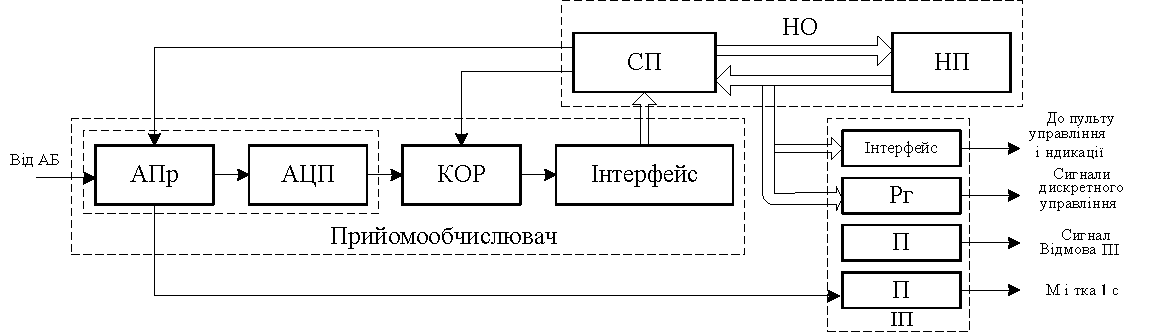
\includegraphics[scale=0.9]{sns}
\caption{Схема прийомообчислювача}
\label{fig:sns}
\end{figure} 



В кореляторі (КОР) у цифровій формі формуються синфазні  і квадратурні  відліки, що є 
основою роботи алгоритмів пошуку сигналів по затримці і частоті спостереження за псевдодальністю, 
фазою сигналу і виділення навігаційного повідомлення.

Навігаційний обчислювач НО є цифровим процесором, у якому реалізується обчислювальний процес 
і керування роботою ПІ. Навігаційний обчислювач зручно представити у виді сигнального процесора 
СП, що реалізує алгоритми первинної обробки квадратурних складових, і навігаційного процесора 
НП, що реалізує алгоритми низькочастотної обробки, тобто рішення навігаційної задачі.

У прийнятого радіосигналу виміряються затримка t або доплерівський зсув частоти \textit{f}доп, 
які є радіонавігаційними параметрами, а відповідні їм дальність до об'єкта\textit{ }Д = \textit{с}t  
і радіальна швидкість зближення \textit{V}p = \textit{f}допl   служать навігаційними параметрами 
(\textit{с }$-$ швидкість світла;  l - довжина хвилі радіосигналу).

Просторове положення споживача визначається в прийомоіндикаторі в два етапи: спочатку визначаються 
поточні координати супутників і первинні навігаційні параметри (дальність, її похідні й ін.) щодо 
відповідних НС, а потім розраховуються вторинні --- географічна широта, довгота, висота споживача і т.д.

Вектор швидкості споживача обчислюють шляхом обробки результатів вимірів доплерівських зсувів 
частоти сигналів НС з урахуванням відомого вектора швидкості супутника. 

Інтерфейсний пристрій (ІП) призначений для забезпечення взаємодії прийомоіндикатора з зовнішніми 
пристроями такими, наприклад, як пульт керування й індикації (ПКІ). Додатково до складу ІП входять 
два підсилювачі П, що формують ознаку відмови ПІ і сигнали дискретного керування, а також 8-розрядний 
регістр Рг, що приймає сигнали дискретного керування. Цей регістр доступний для читання з боку НО. 
Останній, у залежності від інформації, що знаходиться в регістрі, вибирає той або інший режим роботи.

Таким чином, основною операцією, що виконуваної в СНС за допомогою космічного сегменту, сегменту 
керування та сегменту споживача, є визначення просторових координат місця розташування споживачів і 
часу, тобто просторово-тимчасових координат (ПТК). Як було показано, цю операцію здійснюють відповідно 
до концепції незалежної навігації, що передбачає обчислення шуканих навігаційних параметрів 
безпосередньо в апаратурі споживача. У рамках цієї концепції в СРНС обраний позиційний спосіб 
визначення місця розташування споживачів на основі беззапитних (пасивних) далекомірних вимірів по 
сигналах декількох навігаційних штучних супутників Землі з відомими координатами. Висока точність 
визначення місця розташування споживачів обумовлена багатьма факторами, включаючи взаємне розташування 
супутників і параметри їхніх навігаційних сигналів. Структура космічного сегмента забезпечує для 
споживача постійну видимість необхідного числа супутників.




Використання СНС в інтересах місцезнаходження і навігації рухливих об'єктів, а також у рішенні 
спеціальних задач (спостереження, аерофотознімання, пошук корисних копалин, пошук і порятунок 
транспортних засобів, що терплять нещастя, і людей) висуває високі вимоги.

Вимоги до точнісних характеристик, таких як середньоквадратичне відхилення помилки (СКП) визначення 
навігаційних параметрів, показників надійності навігаційного забезпечення, тощо наступні:
\begin{itemize}
  \itemдоступність (готовність),\textit{ }мірою якої є імовірність працездатності СРНС перед виконанням 
тієї або іншої задачі та у процесі її виконання. Чисельні значення доступності складають 0,95...\dots 0,997;

 \itemцілісність\textit{,  }мірою якої є імовірність виявлення відмови протягом часу, рівному заданому 
або менше. Вимоги до цілісності для маршрутних польотів складає 0,999;

 \itemбезперервність обслуговування,\textit{ }мірою якої служить імовірність працездатності системи 
протягом найбільш відповідальних відрізків часу. На етапах заходу на посадку вимоги до безперервності 
обслуговування складають $10^{-5}$ \dots ... $10^{-4}$ для проміжків часу від 15 до 150 с.
\end{itemize}


Основні навігаційні параметри, що визначаються в СРНС -- дальність і радіальна швидкість. Відповідними 
їм радіонавігаційними параметрами (параметрами радіосигналу) служать затримка t сигналу і доплерівський 
зсув частоти $f_\text{доп}$. Оскільки головною вимогою до СРНС є висока точність виміру 
навігаційних параметрів, отже, й основною вимогою до радіосигналів так само є висока точність 
виміру затримки t сигналу і доплерівського зсуву частоти $f_\text{доп}$.

Вимоги до підвищення точності затримки сигналу і доплерівського зсуву частоти суперечливі. 
Для підвищення точності виміру затримки необхідно розширювати спектр сигналу, а для підвищення 
точності виміру  доплерівського зсуву частоти $-$  збільшувати тривалість сигналу.

Дане протиріччя вирішується при вирішенні задачі спільної оцінки t та  $f_\text{доп}$.

Підвищення точності спільних оцінок затримки сигналу і доплерівського зсуву частоти можна 
досягти за рахунок збільшення так званої  бази сигналу -- \textit{В}(добуток ефективної 
тривалості сигналу на ефективну ширину спектра сигналу) і основною вимогою до радіосигналів у 
СРНС є збільшення бази сигналу \textit{В}  1. Такі сигнали називають шумоподібними. 
Відомо, що стійкість до перешкод радіотехнічної системи визначається значенням бази сигналу, 
а для більшості ЛА скритність і перешкодозахищеність є одним з визначальних вимог. 

Інша істотна вимога --- забезпечення багатостанційного доступу. При визначенні навігаційних 
параметрів у споживача повинна бути можливість одночасного доступу до сигналів від різних 
супутників. Проблема багатостанційного доступу вирішується шляхом тимчасового, частотного 
або кодового поділу сигналів, наприклад, у супутниковій навігаційній системі GPS використовується 
кодовий поділ, у СРНС ГЛОНАСС - частотний.

З результатів аналізів стає очевидно, що не має принципової різниці між супутниковими 
навігаційними системами GPS та ГЛОНАСС.

В залежності від області використання апаратура споживача (АС) має свої особливості, 
тому виробники АС завжди вказують на область застосування відповідного зразка. Крім 
основних блоків, таких, як антена, приймач, індикатор, АС може містити допоміжні, що 
забезпечують виконання спеціальних сервісних функцій, наприклад, діагностику вузлів 
транспортного засобу, зв'язок з диспетчерським пунктом і т.п.

В табл. \ref{tb:ac} наведені коротка інформація про основні зразки АС, що працюють за сигналами 
СРНС ГЛОНАСС та GPS. Наведена інформація не претендує на повноту відомостей як про існуючі 
зразки АС, так і про іх характеристики, а дається для ілюстрації досягнутого рівня 
в розробці та виробництві АС СРНС.







Апаратура споживачів
\begin{table}[here]
\small
\caption{Апаратура споживачів}
\centering
\begin{tabular}{|p{30mm}|p{20mm}|p{20mm}|p{20mm}|p{20mm}|p{20mm}|p{10mm}|} \hline 
Найменування апаратури & Область використання & Виробник & Число каналів & 
\multicolumn{2}{|p{30mm}|}{Точність (в автономному режимі)} & Маса, кг \\ \hline 
 &  &  &  & координат, м & швидкості, м/с &  \\ \hline 
Станція моніторингу та формування ДП & Моніторинг & РНИИ КЛ & 24 & 1...3 & 1...2 & 6,0 \\ \hline 
„Гном-М'' & Авіація &  & 6...12 & 80...90 & 12...15 & 3,2 \\ \hline 
АСН-22 & Авіація & РИРВ & 18 & 25...30 &  & 0,4 \\ \hline 
НАВИС СН 3301 & Авіація &  & 14 & 15...20 & 8...10 & 2,4 \\ \hline 
„Интер-А'' & Авіація & МКБ КОМПАС & 12 & 25...30 & 10...30 & 3,5 \\ \hline 
А-744 & Авіація & Фирма „Кодтик'' & 6 & 30...35 & 15...20 & 2,0 \\ \hline 
\end{tabular}
\label{tb:ac}
\end{table}


З огляду на, те що  супутникова система навігації буде працювати в комплексі з 
інерціальною системою навігації, то навряд варто встановлювати  на борт ЛА повний 
комплект супутникової системи. Досить обмежитися  прийомоіндикатором і сигнальним 
процесором, думаючи, що алгоритми рішення навігаційної задачі будуть вирішуватися 
в спільному процесорі інерціально - супутникової системи навігації. 

Виходячи з вищенаведеного, а також враховуючи умови застосування ЛА та вимоги 
ТЗ можна сформулювати вимоги, яким повинний задовольняти обраний тип прийомоіндикатора 
СРНС. 

Розв'язувані задачі:
\begin{itemize}

\item автоматичне, безперервне, глобальне, всепогодне визначення поточних ЗD-координат 
місця розташування, вектора шляхової швидкості шляхового кута ЛА при роботі: по 
сигналу стандартної точності частотного діапазону L1 ГЛОНАСС; по сигналі З/А-коду 
GPS; при спільній обробці вищевказаних сигналів;

\item видача поточних ЗD-координат місця розташування ЛА, що є складовими вектора 
швидкості і шляхового кута в системі координат СК-42 або ПЗ-90 у географічному 
форматі, а також ознак режиму роботи апаратури;

\item стійке визначення навігаційних параметрів при русі з лінійними прискореннями 
і при стрибкоподібних змінах прискорення;

\item  можливість переключення з антени носія на антену ЛА; 

\item інтегральна оцінка очікуваної точності визначення поточних координат місця розташування;

\item автоматичний вибір оптимального з погляду очікуваної точності сузір'я НС ГЛОНАСС і GPS при роботі в сполученому режимі;

\item автоматичне рішення навігаційної задачі в географічній системі координат:  
\end{itemize}

\vspace{5mm}
\textbf{Джерела похибок СНС} \\ 
Визначення координат вимагає точний час, позицію супутників і затримки вимірів 
отриманого сигналу. Точність позиціонування переважно залежить від координат 
супутників і затримки сигналу.Загальним недоліком любої СНС є те, що сигнал при деяких умовах може не доходити 
до приймача, або приходити із значними затримками та спотвореннями. Далі розглянуто 
основні джерела похибок СНС.

\vspace{5mm}
\textit{Вибіркова доступність} \\
Суттєвим недоліком є повна залежність умов отримання сигналу від міністерства 
оборони США у випадку GPS, методом додавання похибки елалону часу супутниками, що 
впливає на визначення координат для не авторизованих користувачів. В травні 2000  
року таке обмеження було знято, але немає гарантії, що це не станеться знову. 
Так, наприклад, під час бойових дій в Іраці, весь цивільний сектор був відключений.

\vspace{5mm}
\textit{Атмосферні явища}\\
Атмосферні ефекти представляються наступними помилками. Тропосфера знаходиться 
на висоті від 6 до 18 км. Вона електрично нейтральна і недисперсна для частот 
до 15 ГГЦ [10,12]. Але через наявність водяного пару, атмосферної температури 
та тиску, спричиняє затримки.

Іоносфера знаходиться на вистоті від 50 до 1500 км і включає велику кількість  
вільних електронів і позитивно заряджених іонів. Це створює групову затримку 
сигналу, а також рефракційні та дифракційні ефекти[10]. Іоносферна 
активність значно залежить від кількості плям на Сонці. Використання деяких 
моделей та DGPS може значно поліпшити визначення координат.

\vspace{5mm}
\textit{Помилки ефемерид та еталону часу}\\
Інше джерело похибок -- це неточність визначення ефемерид. Хоча 
ефемериди і передаються кожні 30 секунд, сама інформація може бути вже 2 
години як застарілою. 

Атомні годинники в супутниках мають бути синхронізовані з часом 
всієї системи. Найменші відхилення моніторяться спеціальними станціями і 
помилка передається як коефіцієнти поліному другого порядку. Більші помилки 
утворються в приймачах і варіюється від мікро- до мілі- секунд.

\vspace{5mm}
\textit{Ефекти відбивання}\\
Сигнали СНС може спотворюватись ефектами не прямолінійності траекторії проходження  
сигналу, де радіосигнал відбивається від навколишнього ландшафту, будинків 
гірської поверхні. Ці затримки сигналу впливають на виміри псевдодальності та фази. 

\vspace{5mm}
\textit{Затримки сигналу}\\
Для виміру затримки, приймач порівнює послідовність бітів, отриманих з супутника, 
з генерованою версією. Через порівняння наростання і спадання імпульсів, сучасна 
електроніка може визначати зміщення сигналу імпульсу кожного біта в межах одного 
відсотку, або приблизно 10 нс для С/А коду. Так як сигнал СНС розповсюджується із 
швидкістю світла, виникає помилка приблизно 3м.
Точність може бути покращена приблизно в 10 разів, за рахунок викорисання 
більш високочастоного сисгналу, помилка зменшуєтья приблизно до 0.3 м.

\vspace{5mm}
\textit{Зниження точності (DOP)}\\
DOP -  зниження точності (англ. Dilution of precision, DOP) - термін, 
що використовується в області систем глобального позиціонування для 
параметричного опису геометричного розташування супутників щодо антени 
приймача. Коли супутники в області видимості знаходяться дуже близько 
один до одного говорять про «слабку» геометрії розташування (високе значення DOP), 
і, навпаки, при достатній віддаленості геометрію вважають «сильною» (низьке значення DOP). 
Фактори, що впливають на геометричне зниження точності.

Орбіти супутників
присутність обєктів перешкод, що затіняють необхідну область неба
вплив атмосфери
відбивання радіохвиль

Поимилки псевдодальностей $ \delta\rho $ може бути отримана з позиційних помилок 
 та помилок еталону часу $\delta e =[\delta x, \delta y, \delta z, c\cdot p\delta t]^T $
% за допомогою лінеаризованого рівняння:
% \begin{equation}
% \label{eq:sns_err}
% \delta\rho = H\deltae + \delta\epsilon_\pho
% \end{equation}
% 
%  де H (m$\times$ 4) матриця частинних похідни по відповідним 4м змінним.
% $\delta\epsilon_\rho$ білий шум з нульовим математичним сподіванням. Приймаючи
% багато спрощень, можливо отримати оцінку вектора $\delta\hat{\epsilon_\rho}$ і
% $E[\delta\hat{\epsilon_\rho} \delta\hat{\epsilon_\rho}^T] = \sigma_\epsilon^2(HH^T)^-1$.
% Перемоноження матриць та інверсію можна представити наступним чином:
% 
% \begin{equation}
% \label{eq:sns_cov}
% \delta\rho = H\deltae + \delta\epsilon_\pho
% \end{equation}



Основні параметри:
\begin{itemize}
 \item HDOP (Horizontal Dilution of Precision) -- зниження точності в горизонтальній площині;
 \item VDOP (Vertical) -- зниження точності у вертикальній площині;
 \item PDOP (Position) -- зниження точності за місцем розташування;
 \item TDOP (Time) -- зниження точності за часом;
 \item GDOP (Geometric) -- геометричне зниження точності.
\end{itemize}



\subsection{Оцінка орієнтовних значень похибок вимірників первинної інформації БІНС}

Датчики первинної інформації БІНС -- датчики кутової швидкості й акселерометри встановлюються жорстко на ЛА. 
Тяжкі умови роботи датчиків інформації призводять до появи значних похибок, тому в алгоритмах роботи БІНС бажано 
здійснити аналітичну компенсацію похибок вимірників (здійснювати їх польотне калібрування), перш ніж ці сигнали 
будуть використані для розрахунку параметрів орієнтації і для визначення складових уявного прискорення уздовж навігаційних осей.

Інструментальні похибки ІНС визначаються погрішностями аmкселерометрів, вимірників кутової швидкості або кута, 
а також погрішностями обчислювального пристрою. Очевидно, при застосуванні обчислювального пристрою досить високої 
точності похибки, ІНС будуть визначатися головним чином погрішностями первинних вимірювальних датчиків, що входять у систему.

Якщо акселерометри ІНС вимірюють прискорення $a_{x} $ і $a_{y} $ з погрішностями $\Delta a_{x} $ і $\Delta a_{y} $, то,  
це приведе до помилки у визначенні координати $\Delta \lambda _{y} $.

Приладові значення зазначених параметрів (зі значком «*»)

\begin{equation} 
\label{eq:err} 
\left. 
\begin{array}{l} 
{a_{\xi }^{*} =a_{\xi } +\Delta a_{\xi } ;{\rm \; \; }a_{x}^{*} =a_{x} +\Delta a_{x} ;{\rm \; \; \; }a_{y}^{*} =a_{y} +\Delta a_{y} ;} 
\\ {\dot{\lambda }_{y}^{*} =\dot{\lambda }_{y} +\Delta \dot{\lambda }_{y} ;{\rm \; \; \; }\lambda _{y}^{*} =\lambda _{y} 
+\Delta \lambda _{y} ;{\rm \; \; \; }}
\\ {\ddot{\vartheta }'^{*} =\ddot{\vartheta }'+\Delta \ddot{\vartheta }'; \dot{\vartheta }'^{*} =\dot{\vartheta }'+\Delta \dot{\vartheta }';
{\rm \; \; \; }\vartheta '^{*} =\vartheta '+\Delta \vartheta '.} \end{array}\right\} 
\end{equation} 

Підставивши значення цих параметрів у перші рівняння систем і зробивши відповідні перетворення наступне рівняння похибок:

\begin{equation} 
\label{eq:lam_err} 
\Delta \ddot{\lambda }_{y} +\frac{(a_{\eta } +g_{0} )}{R_{{\text{З}}} } 
\Delta \lambda _{y} =\frac{1}{R_{{\text{З}}} } \left[a_{x} \cos (\lambda _{y} -\vartheta ')+a_{y} \sin (\lambda _{y} -
\vartheta ')\right] 
\end{equation} 

Як видно, ліва частина рівняння \eqref{eq:lam_err} є (при $a_{\eta } =0$) рівнянням маятника Шулера, а права -- збурюючим впливом.

Координата $\lambda _{y} $ і кут $\vartheta '$ у процесі руху безупинно змінюються, тому права частина рівняння \eqref{eq:lam_err} 
буде теж змінною в часі.

З огляду на вираз і те, що при автоматичному керуванні рухом кут відхилення об'єкта від площини горизонту досить малий, а також вважаючи

\[\Delta a_{x} =\Delta a_{y} =\Delta a\] 

у першому наближенні одержимо

\begin{equation} 
\label{eq:2_51} 
\Delta \ddot{\lambda }_{y} +\frac{1}{R_{{\text{З}}} } (a_{\eta } +g_{0} )\Delta \lambda _{y} \cong \frac{\Delta a}{R_{{\text{З}}} }  
\end{equation} 

При $a_{\eta } =0$, $\Delta a={\rm const}$ рішення рівняння \eqref{eq:2_51} буде наступним:

\begin{equation} 
\label{eq:2_52_} 
\Delta \lambda _{y} \cong \frac{\Delta a}{g_{0} } \left(1-\cos \left(\sqrt{\frac{g_{0} }{R_{{\text{З}}} } } \cdot t\right)\right) 
\end{equation} 

З виразу \eqref{eq:2_52_} видно, що помилка ІНС у визначенні; координати $\lambda _{y} $, обумовлена похибкою акселерометрів, 
буде мати як постійну, так і змінну складові.Найбільше значення похибки не перевищить  $\Delta \lambda _{y} \le 2\frac{\Delta a}{g_{0} } $. 

%Графік залежності $\Delta \lambda \left(t\right)$, отриманий шляхом моделювання однокомпонентної БІНС, при наявності 
%постійних похибок акселерометрів представлений на мал. 2.5, \textit{а}. 

%\includegraphics[bb=0mm 0mm 208mm 296mm, width=86.2mm, height=65.5mm, viewport=3mm 4mm 205mm 292mm]{image1.ps}\includegraphics[bb=0mm 0mm 208mm 296mm, width=84.4mm, height=65.3mm, viewport=3mm 4mm 205mm 292mm]{image2.ps}                   \textit{а)}                                                                          \textit{б)}


\textbf{Оцінка помилки акселерометрів}

За допомогою \eqref{eq:2_52_} можуть бути отримані орієнтовані формули для розрахунку точнісних вимог пропонованих до датчиків первинної 
інформації -- акселерометрам.

\begin{equation} 
\label{eq:acc_err} 
\Delta a\cong \frac{\Delta \lambda _{y} g_{0} }{\left(1-\cos \left(\sqrt{\frac{g_{0} }{R_{{\text{З}}} } } \cdot t\right)\right)}.    
\end{equation} 

Як випливає з \eqref{eq:acc_err} вимоги до точнісних характеристик акселерометрів залежать від проміжків часу 
автономної роботи БІНС у складі комплексної інерціально-супутникової системи навігації. Виходячи з вимог до 
точності визначення координат (СКВ  5 м) отримані орієнтовані значення похибок акселерометра, у залежності 
від очікуваних перерв у роботі супутникової системи навігації. Розрахункові значення точнісних вимоги 
пропонованих до датчиків первинної інформації, зокрема акселерометрів відображені на графіку рис. \ref{fig:acc_err} 

\begin{figure}
\centering
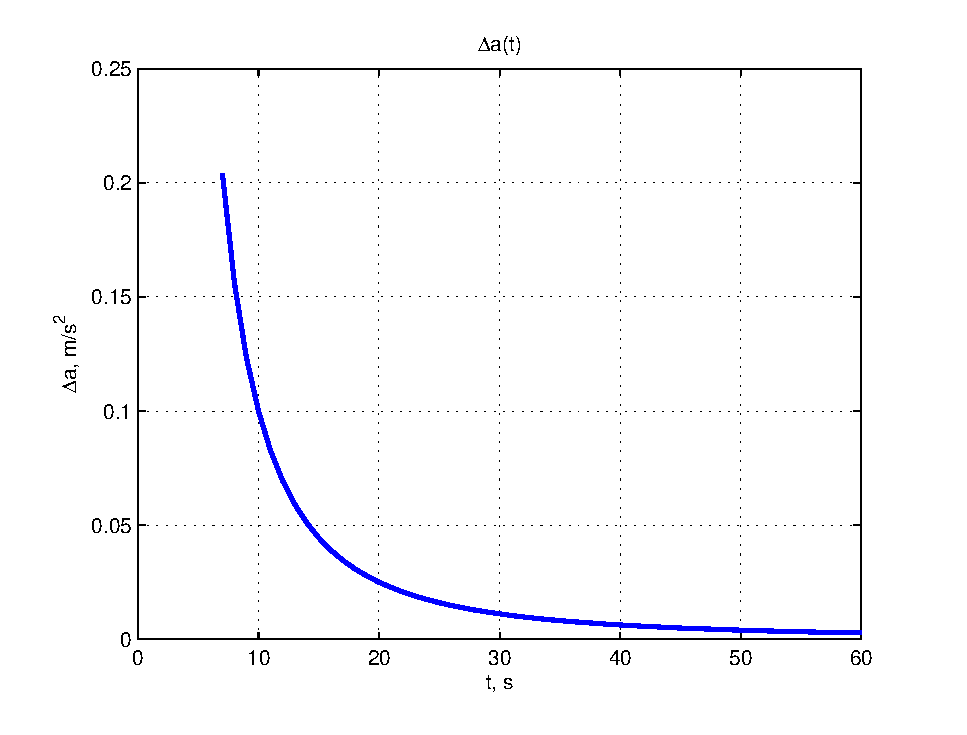
\includegraphics[scale=0.8]{acc_err}
\caption{Графік залежності значень похибок акселерометра від часу}
\label{fig:acc_err}
\end{figure} 
\vline 

\textbf{Оцінка помилки датчика кутової швидкості}

Якщо вимірник кутової швидкості об'єкта має погрішність $\Delta \vartheta '$, то приладове значення кутової швидкості

\[\dot{\vartheta }'^{*} =\dot{\vartheta }'-\Delta \dot{\vartheta }'.\] 

При цьому, будуть мати місце помилки у визначенні інших параметрів.

Підставляючи значення параметрів $\dot{\vartheta }'^{*} $ і  $\lambda _{y}^{*} $ рівняння \eqref{eq:2_51},  
після перетворень з врахуванням другого рівняння системи \eqref{eq:err} одержимо

\begin{equation} 
\label{eq:2_54_} 
\Delta \ddot{\lambda }_{y} +\frac{a_{\eta } +g_{0} }{R_{\text{З}} } \Delta \lambda _{y} =-\frac{a_{\eta } +g_{0} }{R_{\text{З}} } \Delta \vartheta ' 
\end{equation} 

Як видно ліва частина рівняння \eqref{eq:2_54_} і в цьому випадку (при $a_{\eta } =0$) представляється рівняння 
маятника Шулера, а права частина -- фактор, що викликається, обумовленими погрішностями у вимірі $\vartheta '$кута .

Якщо вважати погрішність $\Delta \dot{\vartheta }'=\Delta \dot{\vartheta }'_{0} =const$, то $\Delta \vartheta '=\Delta \dot{\vartheta }'_{0} t$, 
при цьому рішення рівняння 
\eqref{eq:2_54_} буде (якщо $a_{\eta } =0$) наступної:

\begin{equation} 
\label{eq:2_55} 
\Delta \lambda _{y} =\Delta \dot{\vartheta }'_{0} \left(\sqrt{\frac{R_{\text{З}} }{g_{0} } } \sin \sqrt{\frac{g_{0} }{R_{\text{З}} } } \cdot t-t\right)
\end{equation} 


Як видно з виразу \eqref{eq:2_55},  погрішність у визначенні координати  $\lambda _{y} $, обумовлена 
постійною  помилкою  вимірника кутової швидкості, у першому наближенні має дві складові (рис. 2.5,\textit{б)}, 
одна  з яких  росте пропорційно  часу польоту

\[\Delta \lambda _{y0} =\Delta \dot{\vartheta }'_{0} t,\] 

а інша  змінюється з періодом маятника Шулера

\[\Delta \lambda _{y} =\Delta \dot{\vartheta }'_{0} \sqrt{\frac{R_{\text{З}} }{g_{0} } } \sin \sqrt{\frac{g_{0} }{R_{\text{З}} } } \cdot t\] 


Аналогічно \eqref{eq:acc_err} можуть бути отримані орієнтовані формули для розрахунку точносних вимог 
пропонованих до вимірників кутових швидкостей.

\[\Delta \dot{\vartheta }'_{0} =\frac{\Delta \lambda _{y} }{\left(\sqrt{\frac{R_{{\text{З}}} }{g_{0} } } \sin \left(\sqrt{\frac{g_{0} }{R_{{\text{З}}} } } \cdot t\right)-t\right)} \] 

Виходячи з вимог пропонованих до точносних характеристик визначення координат (СКО $\approx$ 5м) 
отримані орієнтовані значення похибок вимірникам кутових швидкостей, у залежності від очікуваних 
перерв у роботі супутникової системи навігації. Розрахункові значення точнісних вимоги пропонованих 
до датчиків первинної інформації, зокрема вимірникам кутових швидкостей відображені на графіку рис.\ref{fig:gyro_err}.

\begin{figure}[here]
\centering
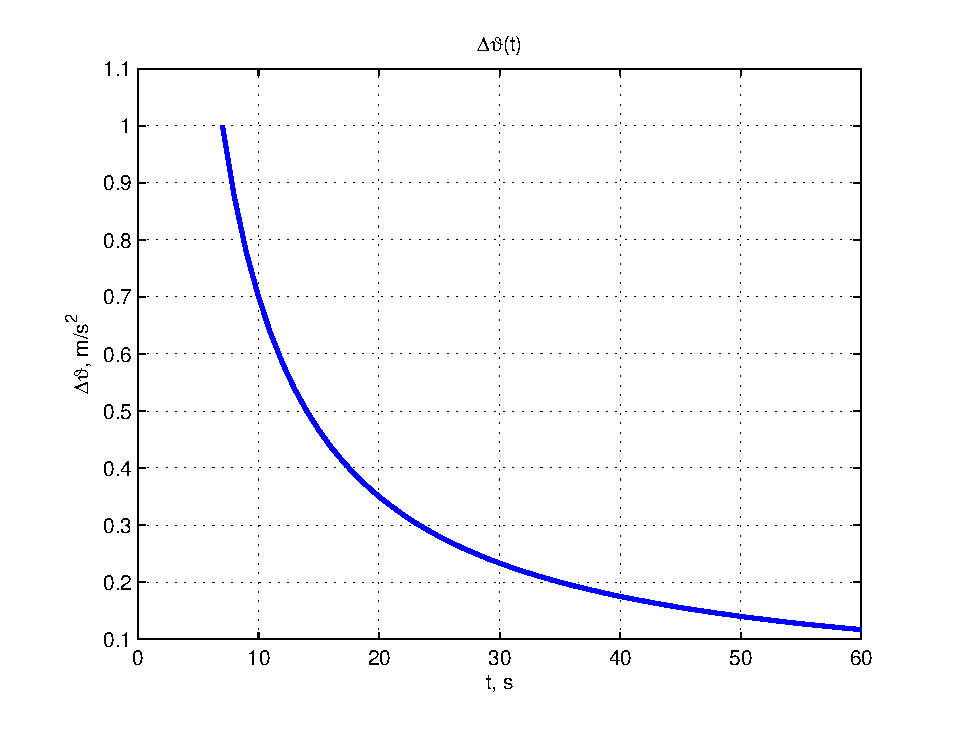
\includegraphics[scale=0.8]{gyro_err}
\caption{Графік залежності значень похибок ДКШ від часу}
\label{fig:gyro_err}
\end{figure} 



% Вихідні похибки БІНС визначаються в основному наступними складовими:
% \begin{enumerate}
%  \item похибками ДКШ і акселерометрів;
%  \item методичними похибками;
%  \item похибками обчислень 
%  \item похибками моделі використовуваної для обліку впливу гравітаційного поля на поводження інерціальних чуттєвих елементів.
% \end{enumerate}


Для БІНС розглянутого класу основний внесок у похибки визначення координат вносять датчики первинної 
інформації. Необхідно відзначити, що методичні похибки, у тому числі похибки, зв'язані зі спрощеннями 
кінематичних рівнянь БІНС, похибками моделювання форми Землі і похибками моделі гравітаційного поля, 
повинні бути не більше  похибок, внесених датчиками первинної інформації.

Багато складові вихідні похибки залежать від параметрів траєкторії й умов роботи, коефіцієнти моделі 
похибок істотно залежать від рівня вібрації і температури. Тому для більш детального дослідження 
точністних характеристик  БІНС необхідна вихідна інформація про аеродинамічні й інерційно масові 
характеристиках літака, а також параметри траєкторії. У цьому випадку можна буде провести детальні 
статистичні дослідження точністних характеристик з урахуванням впливу динамічних похибок датчиків первинної інформації.

Однак при моделюванні враховувалися тільки деякі складові:
\begin{enumerate}
  \itemсистематичні;
  \itemперекручування масштабного коефіцієнта;
  \itemвипадкові складові;
  \itemзони нечутливості
\end{enumerate}

Випадкові складові і перекручування масштабного коефіцієнта моделювалися 
з використанням генераторів "білого шуму" і формуючих фільтрів. При цьому 
вважалося, що кожен чуттєвий елемент цілком визначається значеннями цих 
складових, а самі ці складові змінюються таким чином, що при збільшенні 
одного з них зростають і всі інші. У табл. \ref{tab:gyro_err} та \ref{tab:acc_err}  
показані приклади зміни складових  похибок датчиків первинної інформації.

\begin{table}[here]
\centering
\caption{Параметри акселерометрів}

\begin{tabular}{|p{80mm}|p{20mm}|p{20mm}|p{20mm}|} \hline 
\multicolumn{4}{|p{1in}|}{Акселерометри} \\ \hline 
Зсув показань, $10^{-3}$ & 0,01 & 0,05 & 0,1 \\ \hline 
Масштабний коефіцієнт & 0,001 & 0,005 & 0,01 \\ \hline 
Неортогональність кут.с & 10 & 10 & 20 \\ \hline 
Випадкова складова, м/с3/год & 0,009 & 0,01 & 0,02 \\ \hline 

\end{tabular}
\label{tab:acc_err}
\end{table}


\begin{table}[here]
\centering
\caption{Параметри ДКШ}

\begin{tabular}{|p{80mm}|p{20mm}|p{20mm}|p{20mm}|} \hline
\multicolumn{4}{|p{1in}|}{ДКШ} \\ \hline 
Дрейф, що не залежить від перевантаження, град/год & 0,005 & 0,01 & 0,1 \\ \hline 
Дрейф, що залежить від перевантаження, град/год & 0,0075 & 0,015 & 0,15 \\ \hline 
Масштабний коефіцієнт & 0,0025 & 0,005 & 0,02 \\ \hline 
Неортогональність кут.с & 20 & 60 & 120 \\ \hline 
Випадкове блукання, град/год & 0,0005 & 0,001 & 0,01 \\ \hline 
\end{tabular}
\label{tab:gyro_err}
\end{table}
